\documentclass[a4paper,20pt]{article}

\usepackage{latexsym}
\usepackage[empty]{fullpage}
\usepackage{titlesec}
\usepackage{marvosym}
\usepackage[usenames,dvipsnames]{color}
\usepackage{verbatim}
\usepackage{enumitem}
\usepackage[pdftex]{hyperref}
\usepackage{fancyhdr,graphicx}

\pagestyle{fancy}
\fancyhf{} % clear all header and footer fields
\fancyfoot{}
\renewcommand{\headrulewidth}{0pt}
\renewcommand{\footrulewidth}{0pt}

% Adjust margins
\addtolength{\oddsidemargin}{-0.500in}
\addtolength{\evensidemargin}{-0.500in}
\addtolength{\textwidth}{1in}
\addtolength{\topmargin}{-.45in}
\addtolength{\textheight}{1in}

\urlstyle{rm}

\raggedbottom
\raggedright
\setlength{\tabcolsep}{0in}

% Sections formatting
\titleformat{\section}{
	\vspace{-10pt}\scshape\raggedright\Large
}{}{0em}{}[\color{black}\titlerule \vspace{-6pt}]

%-------------------------
% Custom commands
\newcommand{\resumeItem}[2]{
	\item{
		\textbf{#1}{ #2 \vspace{-2pt}}
	}
}

\newcommand{\resumeItemWithoutTitle}[1]{
	\item{
		{\vspace{-2pt}}
	}
}

\newcommand{\resumeSubheading}[4]{
	\vspace{-1pt}\item
	\begin{tabular*}{0.97\textwidth}{l@{\extracolsep{\fill}}r}
		\textbf{#1} & #2 \\
		\textit{#3} & \textit{#4} \\
	\end{tabular*}\vspace{-5pt}
}


\newcommand{\resumeSubItem}[3]{	\item{
		\begin{tabular*}{0.99\linewidth}{ll@{\extracolsep{\fill}}r}
			\textbf{#1} & #2 &  \textit{#3}
			\end{tabular*}\vspace{-5pt}
		}}

\renewcommand{\labelitemii}{$\circ$}

\newcommand{\resumeSubHeadingListStart}{\begin{itemize}[leftmargin=*]}
	\newcommand{\resumeSubHeadingListEnd}{\end{itemize}}
\newcommand{\resumeItemListStart}{\vspace{-.5pt}\begin{itemize}}
	\newcommand{\resumeItemListEnd}{\end{itemize}\vspace{-5pt}}

\newcounter{pubcounter}
%-----------------------------
%%%%%%  CV STARTS HERE  %%%%%%

\begin{document}
	
	%----------HEADING-----------------
	\begin{minipage}{0.2\textwidth}
		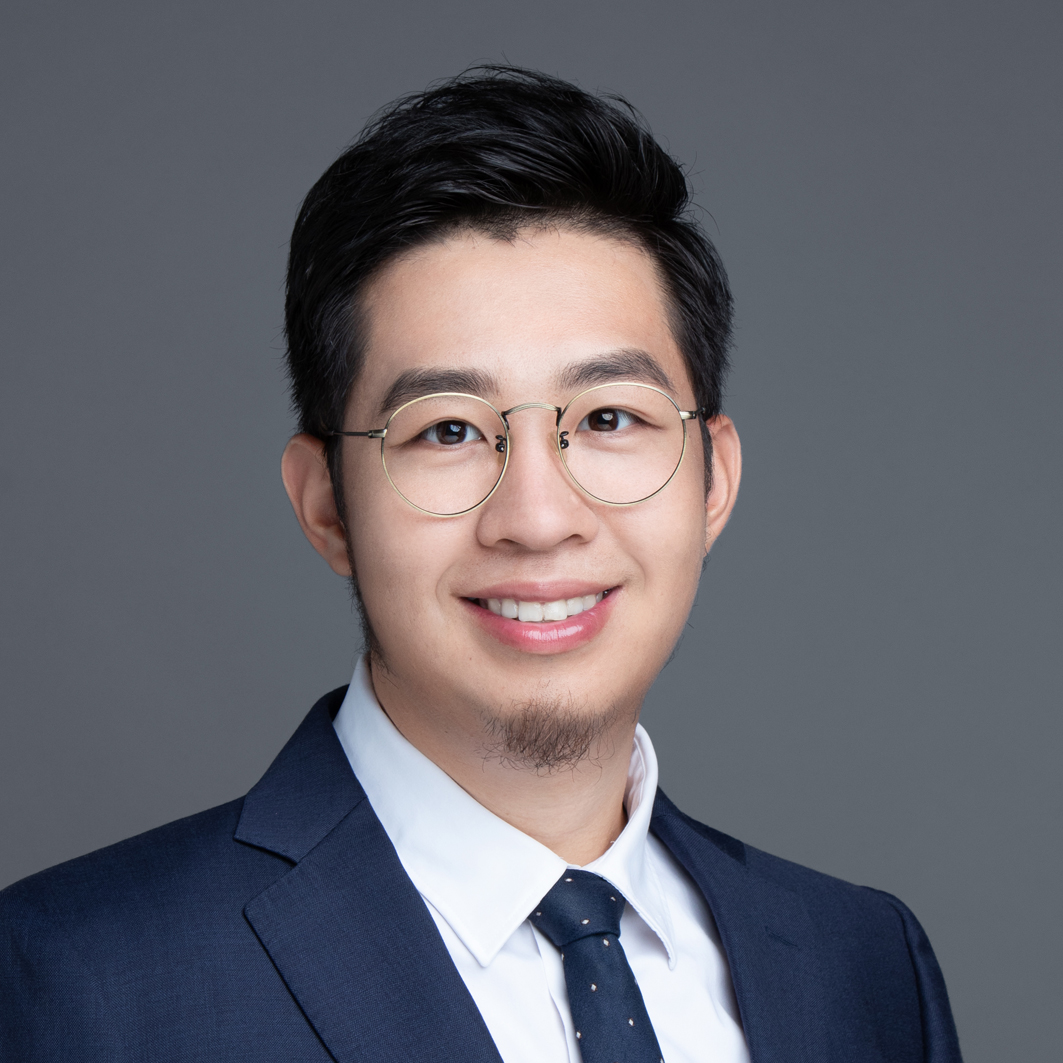
\includegraphics[width=\linewidth]{wang_square}
	\end{minipage}~\hspace{1em}
\begin{minipage}{0.5 \textwidth}
	\textbf{{\LARGE Zhongjian Wang}} \\
	William H. Kruskal Instructor\\
	Department of Statistics and CCAM
	\\
	The University of Chicago 
\end{minipage}~
\begin{minipage}{0.3\textwidth}

		\href{http://www.wangzhongjian.com}{Website: wangzhongjian.com} \\ Mobile:~~~+1-347-506-5855 \\
	Email: \href{mailto:}{zhongjian@uchicago.edu}
\end{minipage}
\\
\hspace{2em}
\\
\textbf{Self introduction:}
For the first thirty years of my life, I am keen on modeling real-world phenomena with math models and developing accurate numerical algorithms to recover and predict them. Now I am seeking a life-changing opportunity to work on more practical math applications in the area of economics, financial markets, and engineering. 
	\section{Employment}
		\resumeSubHeadingListStart
	\resumeSubheading{The University of Chicago, Department of Statistics and CCAM}{Chicago}{William H. Kruskal Instructor, Mentor: Prof. Guillaume Bal}{2020-present}

	\resumeSubHeadingListEnd
	%-----------EDUCATION-----------------
	\section{Education}
	\resumeSubHeadingListStart
	\resumeSubheading
	{The University of Hong Kong, Department of Mathematics}{Hong Kong}
	{Doctor of Philosophy - Supervisor: Prof. Zhang Zhiwen}{2016--2020}
	{}
	\resumeSubheading
	{Tsinghua University, Department of Mathematical Sciences}{Beijing}
	{Bachelor of Science}{2012--2016}

	\resumeSubHeadingListEnd
	\section{Visiting}
\resumeSubHeadingListStart
\resumeSubheading{Tsinghua University}{Beijing}
{Visiting Ph.D. Student, hosted by Professor Steven Shing Tung Yau}{2018.11-19.1}

\resumeSubheading{California Institute of Technology}{Pasadena}
{Visiting Ph.D. Student, hosted by Professor Thomas Hou}{2018.4-5}

\resumeSubheading{Ecole Normale Superieure}{Paris}
{For Bachelor Thesis, supervised by Professor Espen Robstad Jakobsen}{2016.1-6}

\resumeSubheading{University of Oxford}{Oxford}{Tsinghua University Distinguished Newcomer Student Leadership Program}{2013.7}

\resumeSubHeadingListEnd
	\section{Awards}
\resumeSubHeadingListStart
\resumeSubItem{Best PhD thesis Award }{ Hong Kong Mathematical Society}{2021}
\resumeSubItem{Student Travel Award for UQ20 }{ Department of Mathematics, HKU}{2019}
\resumeSubItem{Student Travel Award for CSE19 }{ Society for Industrial and Applied Mathematics}{2019}
\resumeSubItem{Pilot Scheme on International Experience }{ Faculty of Science, HKU}{2017}
\resumeSubItem{IPAM Student Travel Support }{ Institute for Pure \& Applied Mathematics, UCLA}{2017}
\resumeSubItem{Hong Kong Ph.D. Fellowship }{ Research Grants Council of HK}{2016}
\resumeSubItem{Scholarship for Academic Excellence }{ Tsinghua University}{2013}
\resumeSubItem{Gold Medalist }{ China Mathematics Olympiad}{2012}
\resumeSubHeadingListEnd
\section{Services}
\resumeSubHeadingListStart
\resumeSubItem{Captain }{UChicago Chinese soccer team}{2022}
\resumeSubItem{Faculty Sponsor }{CAM Grad Student Seminar}{Chicago, 2021.1-3}
\resumeSubItem{Co-organizer }{Big Data Challenges for Predictive Modeling of Complex Systems}{HK, 2018.11}
\resumeSubItem{Student Representative }{ Lap Chee College of HKU}{HK, 2018-2020}
\resumeSubItem{Founding Captain }{CSSA HKU soccer team}{2018}
\resumeSubItem{Journal Referee }{ Computers and Mathematics with Applications}{}
\resumeSubItem{Memberships }{IEEE, SIAM}{}
\resumeSubHeadingListEnd
	\section{Skills}
\resumeSubHeadingListStart
\resumeItem{Language: }{Chinese, native speaker; English, proficient; Cantonese, beginner.}
\resumeItem{Programming: }{proficient in Matlab, Python, R; beginner in C++.}
\resumeItem{Business: }{Word, Excel, Powerpoint, LaTex}
\resumeSubHeadingListEnd
	\section{Projects}
	Here I will list some of my research projects that have real world applications.
	\resumeSubHeadingListStart
		\resumeSubItem{Inverse Problems}{}{since 2020}
		\vspace{-.5em}\\
		\textbf{Role:} theoretic analysis, programming.\\
		The project aims to find initial condition / source of parabolic PDE. Our studies give the optimal choice of regularization factor during inversion. The methodologies applies to any time evolution  models that need to find starting (or intermediate) state from noisy observation of final state.\\
		 \textsl{Main collaborator: Wenlong Zhang at SusTech.} 
	\resumeSubItem{Machine Learning Algorithms}{ }{since 2018}
			\vspace{-.5em}\\
				\textbf{Role:} model development, algorithm development, programming.\\
			There are several projects on this topic. The common goal of these projects is to utilize the newly introduced machine learning algorithms to solve math problems. We are interested in developing a new network that best fits the inherent structures preserved by the models. Related real-world models include the Cucker-Smale model which describes the flocking behaviors of sheep and people; the Keller Segel model to describe the formulation of the tumor, etc.\\
			\textsl{Collaborators: Jack Xin at UCI, Zhiwen Zhang at HKU, Yuehaw Khoo at UChicago}\\
	\resumeSubItem{Non-Linear Filtering}{}{since 2017}
	\vspace{-.5em}\\
		\textbf{Role:} algorithm development, programming\\
		The name of non-linear filtering comes from the non-linearity of the dynamics and the observations. The posterior of the state is no longer Gaussian and hence we cannot use two statistics (mean and standard derivation) to fully describe it. Zakai equation is a PDE of the posterior density function. Our projects are to design fast algorithms to solve it in a real-time manner. These projects find applications in the real-time detection of the signal, especially when the observation is non-linear.  \\
	\textsl{Collaborators: Stephen Shing-Tung Yau at Tsinghua}\\
	\resumeSubItem{Monte Carlo simulation}{ }{since 2015}
	\vspace{-.5em}\\
\textbf{Role:} theoretic analysis, programming.\\
This is the main line of my research ever since my undergrad.  I am interested in the accuracy of the long-time Monte Carlo simulation. The theme of every project is to develop SDE schemes that can simulate dynamics for infinite time without accumulation of error. In this way, we can characterize features of dynamic flows without solving PDEs. Applications of Monte Carlo simulation include, option pricing, weather prediction, etc. \\ 
	\textsl{Collaborators: Jack Xin at UCI, Zhiwen Zhang at HKU}\\
	\resumeSubHeadingListEnd
%-----------Awards-----------------

	\section{Publications}
	\textsl{(Names in Math papers are arranged in alphabetical order.)}
	\begin{enumerate}
		\item{ Li, S., Wang, Z., Yau, S. S. T., Zhang, Z.,Tensor train method for high-dimensional nonlinear filtering problems, IEEE Transactions on Automatic Control, 2023.}
		\item{Wang, Z., Xin, J., Zhang, Z., DeepParticle: learning invariant measure by a deep neural network minimizing Wasserstein distance on data generated from an interacting particle method, Journal of Computational Physics (2022): 111309.}
		\item{Wang, Z., Xin, J., Zhang, Z., Computing effective diffusivities in 3D time-dependent chaotic flows with a convergent Lagrangian numerical method, ESAIM: M2AN 56 (2022) 1521–1544}
		\item{ Lyu, J., Wang, Z., Xin, J., Zhang, Z., A convergent interacting particle method and computation of KPP front speeds in chaotic flows, SIAM Journal on Numerical Analysis, 2022, 60(3): 1136-1167}
		\item{Wang, Z., Xin, J., Zhang, Z., Sharp uniform in time error estimate on a stochastic structure-preserving Lagrangian method and computation of effective diffusivity in 3D chaotic flows, Multiscale Model and Simulation, 19 (2021), no. 3, 1167–1189}
		\item{ Lyu, J., Wang, Z., Xin, J., Zhang, Z., Convergence of stochastic structure-preserving schemes for computing effective diffusivity in random flows, SIAM Journal on Numerical Analysis, 58 (2020), no. 5, 3040–3067. .}
		\item{Wang, Z., Zhang, Z., A new mesh-free method for PDE with discontinuous coeffcients using the deep learning approach,  Journal of Computational Physics (2020): 108963.}
		\item{Wang, Z. Luo, X., Yau, S. S. T., Zhang, Z., Proper orthogonal decomposition method to nonlinear filtering problems in medium-high dimension, IEEE Transactions on Automatic Control, 65 (2020), no. 4, 1613–1624.}
		\item{Wang, Z., Xin, J., Zhang, Z.,  Computing Effective Diffusivity of Chaotic and Stochastic Flows Using Structure-Preserving Schemes. SIAM Journal on Numerical Analysis, 56(4), 2322-2344.}
		\setcounter{pubcounter}{\value{enumi}}
	\end{enumerate}
\end{document}
	\resumeSubHeadingListStart
	\resumeSubItem{Research Interests}{}{}

Applied analysis and computational methods for physics and engineering problems, including but not limited to,
\vspace{-5pt}
\resumeItemListStart
\resumeItem{neuron net models:}{transport maps, multiscale physic problems, scattering matrices;}
\resumeItem{data-driven model reduction:}{conditional density function in filtering, uniform accuracy schemes in time integration, inverse problems.}
\resumeItem{structure preserving schemes:}{Lagrangian approach for effective diffusivities, KPP front wave speed; scattering in topological insulators;}
\resumeItemListEnd
	\resumeSubItem{Publications}{}{}

 9 published papers, they are all Tier 1 journals in the related field. In addition, there are currently 5 papers under review. List of journals:
 \vspace{-0.5em}
 \resumeItemListStart
 \resumeItem{SIAM Journal on Numerical Analysis}{(3)}
 \resumeItem{Journal of Computational Physics}{(2)}
 \resumeItem{IEEE Transaction on Automatic Control}{(2)}
 \resumeItem{ESIAM:M2AN}{(1)}
 \resumeItem{Multiscale Models and Simulation}{(1)}
 \resumeItemListEnd
%-----------PROJECTS-----------------
\resumeSubItem{Teaching Experiences}{}{}
 \vspace{-1em}
\resumeItemListStart
	\resumeSubItem{The University of Chicago}{}{2020-present}
\\\vspace{0.5em}
  Lecturer of courses: STAT31120 Numerical Methods for Stochastic Differential Equation, STAT251 Introduction to Probabilities, MATH185 Mathematical Methods in the Physical Sciences (III, ODE)
	\resumeSubItem{The University of Hong Kong}{}{2016-2020}
	\\\vspace{0.5em}
Tutor of courses: MATH3601 Numrical analysis, MATH4602 Scientific computing, MATH2014 Multivariable calculus and linear algebra, MATH1009 Basic mathematics for business and economics
	  \resumeSubItem{Co-Supervising Students}{}{}
	  \\\vspace{0.5em}
List of students: Boyi Hu, Tan Zhang, (with Zhiwen Zhang); Rapha\"{e}l Terrine, Binglu Chen, (with Guillaume Bal)
\resumeItemListEnd
\resumeSubItem{Presentations}{}{}

Invited to present research progress in the following:
\vspace{-.5em}
\resumeItemListStart
\resumeItem{Greater China}{}  

SusTech, BUAA, HKU. Conferences: ICCM 19 at Beijing, AIMS 18 at Taibei
\resumeItem{United States}{}  

UChicago, Columbia, UCLA, IIT, Purdue. Conferences: SIAM UQ22 at Atlanta, SIAM CSE19 at Spokane
\resumeItem{Europe}{} 

EPFL, ENPC. Conference: ICIAM 2019 at Valencia.
\resumeItemListEnd
\resumeSubItem{Academic Referee}{}{}
\vspace{-1.2em}
\resumeItemListStart
\resumeItem{Guillaume Bal}{University of Chicago}
\resumeItem{Jack Xin}{University of California, Irvine}
\resumeItem{Thomas Hou}{Caltech}
\resumeItem{Stephen S.T. Yau}{Tsinghua}
\resumeItem{Zhiwen Zhang}{HKU}
\resumeItemListEnd
	\resumeSubHeadingListEnd

\end{document}